% chapters/prologo.tex
\cleardoublepage
\chapter*{Prologo. Lacrime in cameretta}
\markboth{Prologo}{Prologo}

Alice è arrabbiata, risentita, offesa, triste e amareggiata, per questo le lacrime le stanno rigando gli occhi.
Soffre, ma non darà a sua madre la soddisfazione di vederla così.
Resta chiusa in camera, al riparo senza che nessuno possa vedere, minimizzare, giudicare.
Prende un quaderno, una penna e la chitarra che le ha regalato suo padre dopo il saggio di flauto: «Ora impara con questa» le aveva detto. %

Non l'ha studiata molto, ma conosce gli accordi principali e, nonostante i tempi, sa come si scrive una canzone.
Non solo: sa come si scrive un testo; non uno di quelli più o meno scontati che si trovano in streaming, ma un testo che sa parlare a una sola persona, che sa avvicinarla con delicatezza, farle aprire le porte del cuore per poi piantarci un coltello. %
Già, proprio come ha fatto Caterina con lei.

\begin{figure}[H]
  \centering
  \includegraphics[width=.35\linewidth]{diario alice senza sfondo.png}
  %\caption*{\footnotesize Le parole della canzone sul quaderno di Alice, con accordi per la chitarra.}
\end{figure}

Questa qua sotto è Alice, quasi grande ma ancora adolescente; a vederla nel suo vestitino skater non sembra capace di parole così taglienti.

\begin{figure}[H]
  \centering
  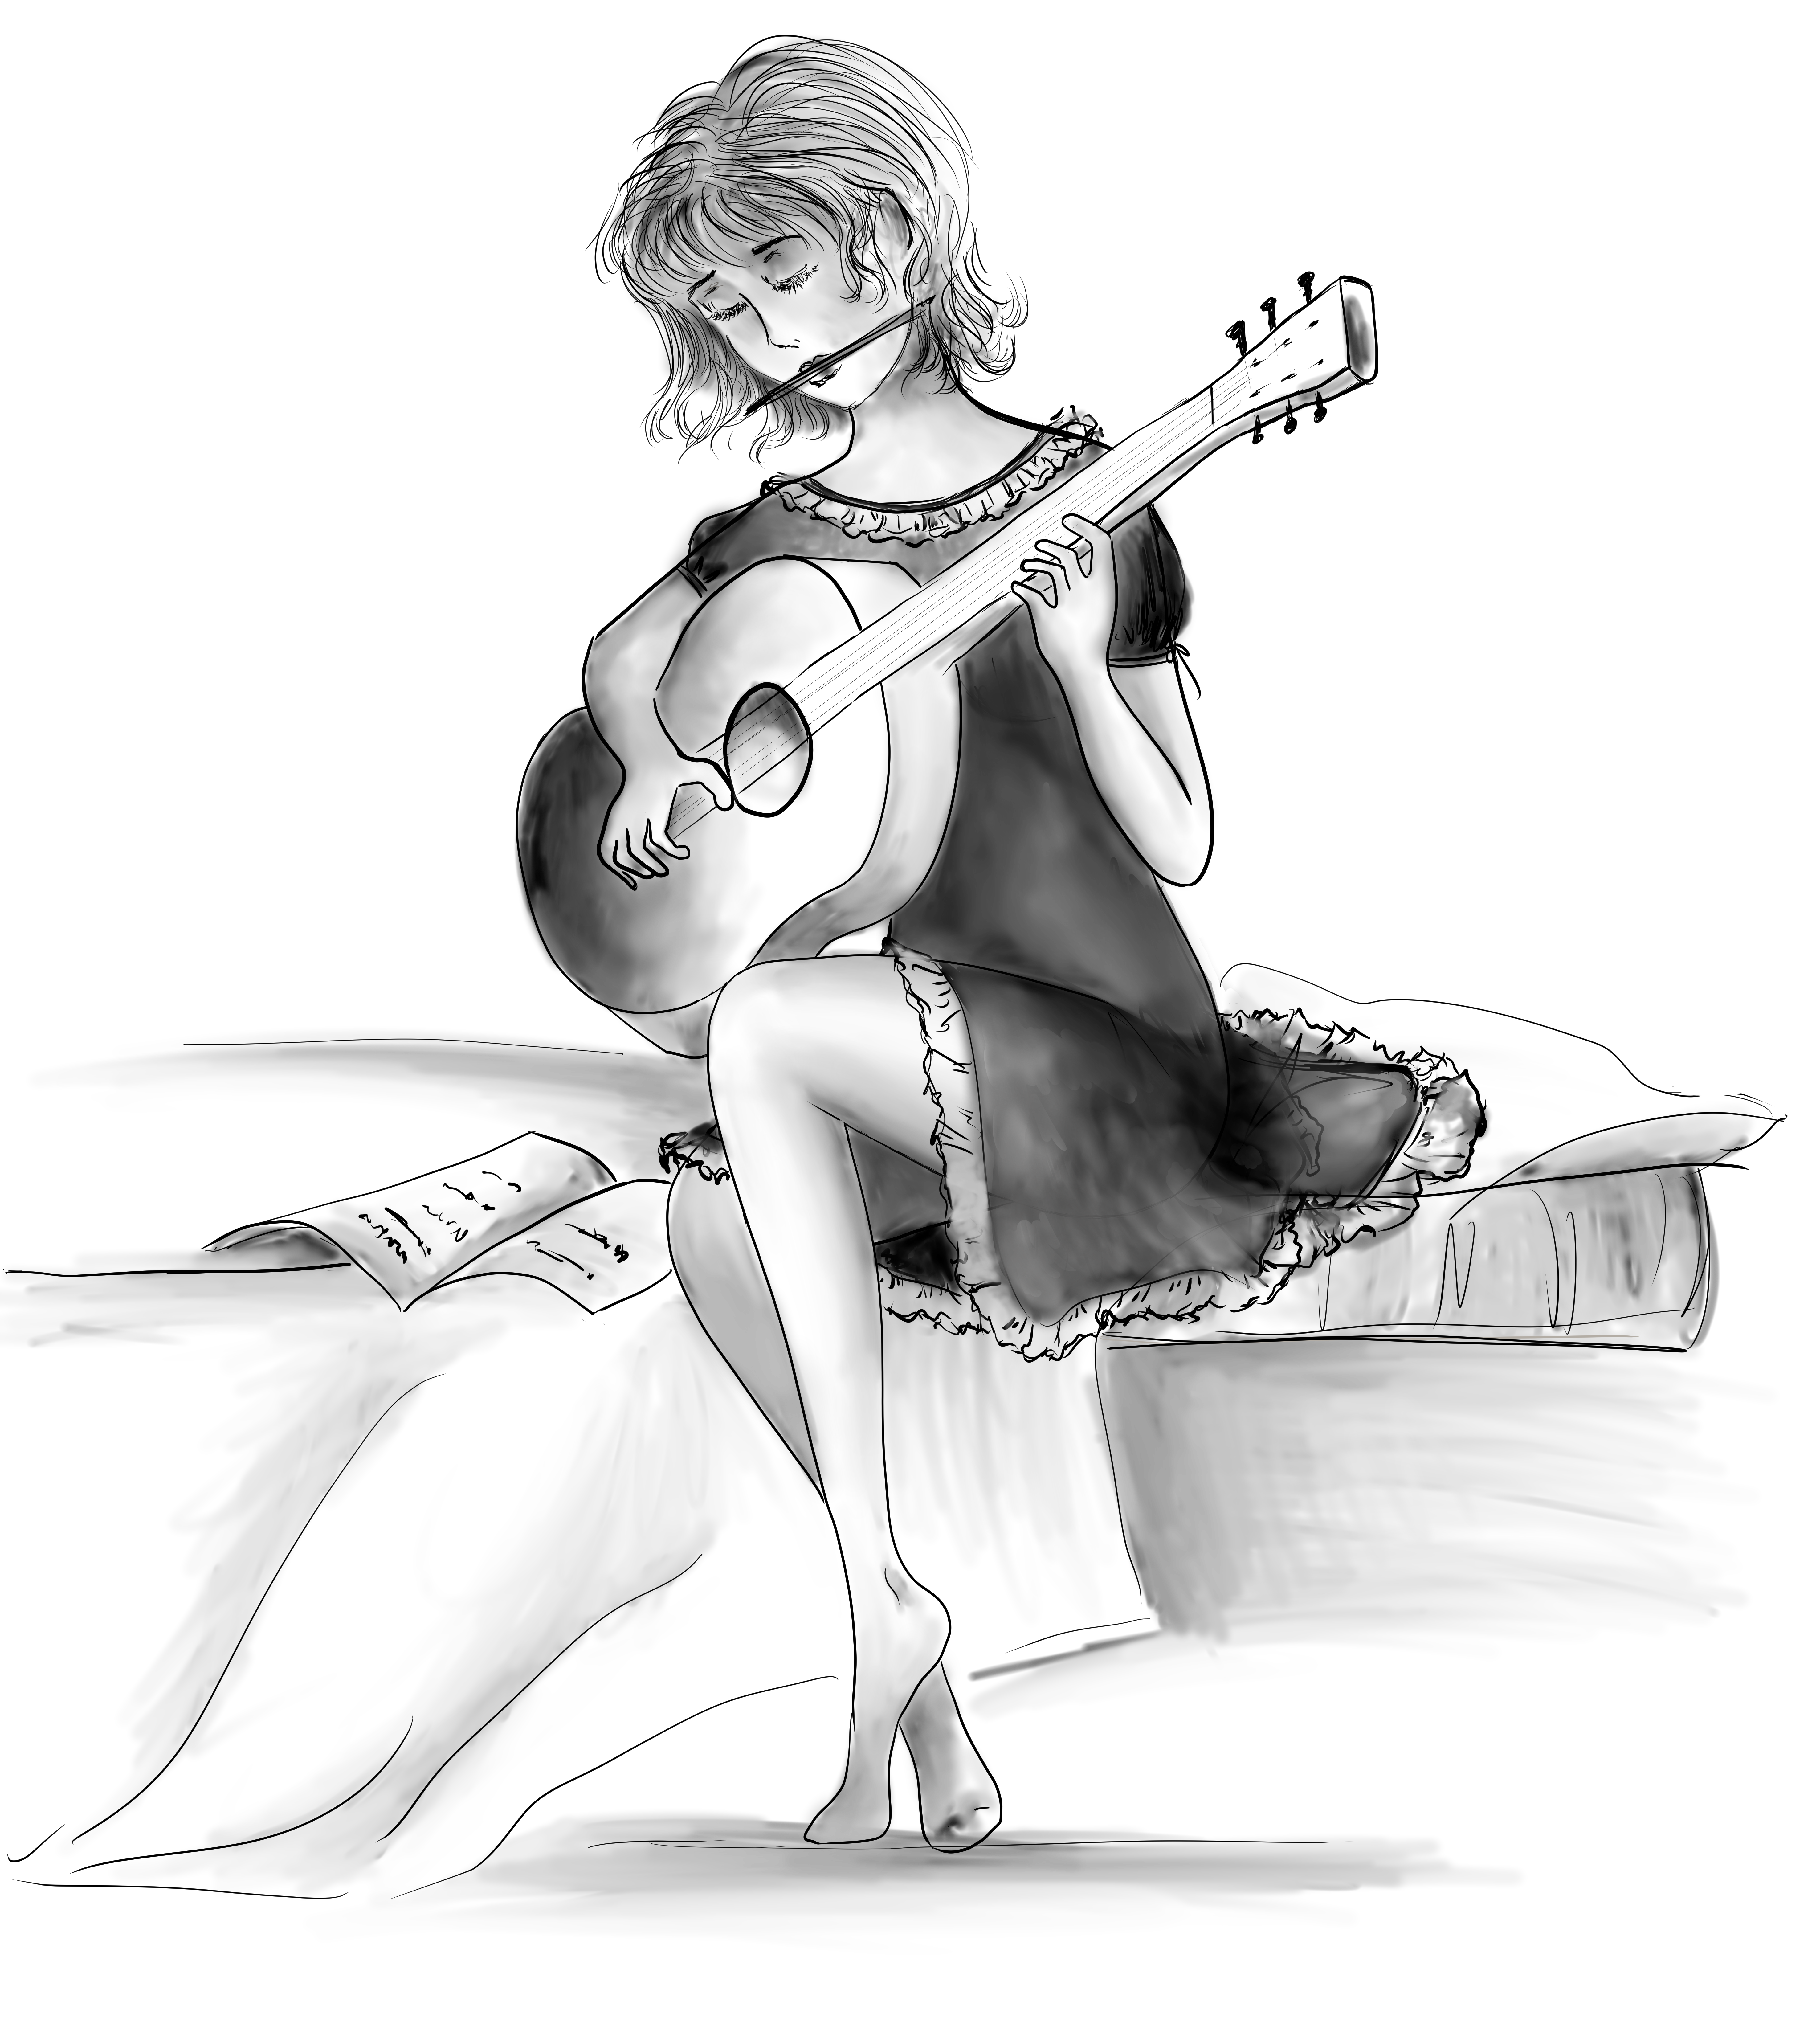
\includegraphics[width=.35\linewidth]{alice senza sfondo.png}
  %\caption*{\footnotesize Alice piange mentre suona la sua canzone.}
\end{figure}
